\documentclass[conference]{IEEEtran}
\IEEEoverridecommandlockouts
% The preceding line is only needed to identify funding in the first footnote. If that is unneeded, please comment it out.
\usepackage{cite}
\usepackage{amsmath,amssymb,amsfonts}
\usepackage{algorithmic}
\usepackage{graphicx}
\usepackage{textcomp}
\usepackage{xcolor}
\usepackage{float}
\def\BibTeX{{\rm B\kern-.05em{\sc i\kern-.025em b}\kern-.08em
    T\kern-.1667em\lower.7ex\hbox{E}\kern-.125emX}}
\begin{document}

\title{BUILDING A REAL-TIME SPEECH EXTRACTION, SUMMARIZATION, AND TRANSLATION SYSTEM THROUGH THE INTEGRATION OF MACHINE LEARNING MODELS\\
}

\author{
    \IEEEauthorblockN{1\textsuperscript{st} Cao Hoài Sang}
    \IEEEauthorblockA{\textit{Department of Information Systems} \\
        \textit{University of Information Technology}\\
        Ho Chi Minh city, Viet Nam \\
        21522541@gm.uit.edu.vn}
    \and
    \IEEEauthorblockN{2\textsuperscript{nd} Cao Hoài Sang}
    \IEEEauthorblockA{\textit{Department of Information Systems} \\
        \textit{University of Information Technology}\\
        Ho Chi Minh city, Viet Nam \\
        21522541@gm.uit.edu.vn}
}

\maketitle

\begin{abstract}
    This document is a model and instructions for \LaTeX.
    This and the IEEEtran.cls file define the components of your paper [title, text, heads, etc.]. *CRITICAL: Do Not Use Symbols, Special Characters, Footnotes,
    or Math in Paper Title or Abstract.
\end{abstract}

\begin{IEEEkeywords}
    component, formatting, style, styling, insert
\end{IEEEkeywords}

\section{Introduction}
In the context of increasingly common online meetings and interactions, the need for real-time speech processing and analysis has become urgent. Current speech recognition systems primarily focus on converting speech into text but do not fully support advanced functions such as speaker differentiation, individual conversation summarization, and real-time language translation.

This research aims to develop a real-time speech processing system that integrates multiple functionalities: speaker identification, conversation analysis, and summarization on a per-person basis, while also translating speech into another language without losing the original voice characteristics. The system will apply modern deep learning models in combination with acoustic features to achieve high performance.



\section{Related Work}

In the field of real-time speech recognition and analysis, multiple approaches have been proposed with the aid of machine learning and deep learning techniques. This section presents an overview of the relevant approaches, divided into groups based on the characteristic methodology and the model used.

\subsection{Mel-Frequency Cepstral Coefficients (MFCC)}

MFCC is one of the most common features in speech signal processing. The article on the use of MFCC to extract characteristics for training HMM models (hidden Markov models) by Rabiner~\cite{rabiner1989tutorial} detailed the use of hidden Markov models (HMM) combined with MFCC characteristics for speech recognition.
\subsection{Wavelet-based Features}

Wavelet transform is a powerful tool used to exploit time and frequency information from audio signals. Wavelet shows good ability to handle sound in noisy or unstable environments. Although not as widely available as MFCC, wavelets have recently been applied to systems thanks to their powerful noise cancellation capabilities. Studies have shown that using wavelet transforms in feature extraction can improve the accuracy of speech recognition systems, particularly in environments with noise \cite{gupta2003robust, wang2008robust}.

\subsection{X-vector and D-vector Embeddings}

X-vectors and D-vectors are representations learned from audio data, often used for speaker recognition. X-vector systems often use DNN or TDNN networks to learn performances to improve speaker discrimination accuracy. These representations are widely used in modern processing, for example in the systems of Kaldi and SpeechBrain. Snyder et al.~\cite{Snyder2018Xvectors} introduced X-vector as a deep learning representation for speaker recognition. For D-vector, Wan et al.~\cite{Wan2018Generalized} proposed using the GE2E loss function for training, which improves performance in speaker recognition.

\subsection{Hidden Markov Models (HMM)}

HMM is the foundation of many traditional ASR systems. Rabiner \cite{rabiner1989tutorial} has proposed effective Viterbi training methods and algorithms for HMM in speech recognition. Hybrid systems such as in~\cite{voll2007hybrid, perero2022comparison} also show that combining HMM with neural networks improves accuracy in real-world environments.

\subsection{Recurrent Neural Networks (RNN)}

RNN is a popular model in ASR because it can capture temporal dependencies in speech data. LSTM and GRU variants help solve vanishing gradient problems and are effective in modeling long-term context. Systems like Deep Speech~\cite{hannun2014deep} and work from Graves et al.~\cite{graves2013speech} show that RNN-based models can achieve good results in end-to-end ASR tasks.

\subsection{Quantum Convolutional Neural Networks (QCNN)}

QCNN is a new model in quantum deep learning, proposed to take advantage of quantum properties to reduce the number of redundant parameters, focus on key characteristics, and enhance representability. Cong et al.~\cite{Cong2019QuantumCNN} introduced QCNN as a new quantum machine learning model, which combines with the characteristics of convolutional neural networks and quantum properties to classify quantum states. Although QCNN has not been widely applied in ASR, research by Yang et al.~\cite{Yang2021Decentralizing} has shown potential in combining QCNN with other

\subsection{Resource}
\subsubsection{Dataset}
The dataset used for training and evaluating the speech recognition system consists of a series of Vietnamese conversations collected from various sources. These data sources include natural conversations, group discussions, podcasts, lectures, as well as direct interviews. The dataset reflects the diversity of voices, expressions, and speaking speeds of individual speakers, which helps the model learn the phonetic, prosodic, and pronunciation features of speakers in various contexts.

\subsubsection{Descriptive Statistics}
The total size of the dataset is 15GB, with many measurements listed below:
\begin{table}[h]
    \centering
    \caption{Overview of speech dataset statistics}
    \begin{tabular}{|l|c|}
        \hline
        \textbf{Statistic}                  & \textbf{Value}               \\
        \hline
        Total number of speakers            & 83                           \\
        Total number of dialogues           & 10,430                       \\
        Number of speaker changes           & 751                          \\
        Total number of audio files         & 85                           \\
        Total number of script files (.txt) & 85                           \\
        Total duration of dataset           & 64,608 seconds (17.93 hours) \\
        Average dialogue length             & 6.19 seconds                 \\
        Standard deviation of length        & 11.96 seconds                \\
        \hline
    \end{tabular}
\end{table}
\subsection{Methodology}
\subsubsection{Hidden Markov Model (HMM) - Mel Frequency Cepstral Coefficients (MFCCs)}
HMM is a probabilistic model used to describe a sequence of observations $O = \{o_1, o_2, ..., o_T\}$ through a set of hidden states $Q = \{q_1, q_2, ..., q_N\}$.

An HMM is defined by three main parameters:
\begin{itemize}
    \item $A = [a_{ij}]$: The state transition probability matrix, where $a_{ij} = P(q_{t+1} = j \mid q_t = i)$.
    \item $B = [b_j(o_t)]$: The observation (output) probability, where $b_j(o_t) = P(o_t \mid q_t = j)$.
    \item $\pi = [\pi_i]$: The initial state distribution, $\pi_i = P(q_1 = i)$.
\end{itemize}

In ASR, each word or phoneme can be modeled by an individual HMM. When a speech signal sequence is input, the goal is to find the optimal state sequence $Q^*$ that maximizes the observation probability:
\begin{equation}
    Q^* = \arg\max_Q P(O \mid Q, \lambda)
\end{equation}
where $\lambda = (A, B, \pi)$ are the parameters of the HMM.

The Viterbi algorithm is essential for finding the most likely state sequence based on the HMM. The maximum probability for state $j$ at time $t$ is computed as:
\begin{equation}
    \delta_t(j) = \max_i \left[ \delta_{t-1}(i) a_{ij} \right] b_j(o_t)
\end{equation}

To train the HMM, the Baum-Welch algorithm (a variant of Expectation-Maximization) is used to estimate the parameters:
\begin{equation}
    a_{ij} = \frac{\sum_{t=1}^{T-1} P(q_t = i, q_{t+1} = j \mid O, \lambda)}{\sum_{t=1}^{T-1} P(q_t = i \mid O, \lambda)}
\end{equation}

Mel-Frequency Cepstral Coefficients (MFCC) are widely used in ASR systems to extract speech features by mimicking human auditory perception. The analog speech signal is first digitized, then passed through a high-pass filter and windowed to minimize noise and spectral leakage. The Discrete Fourier Transform (DFT) converts the signal to the frequency domain, which is then mapped to the Mel scale. A logarithmic function is applied to compress the dynamic range, and the Discrete Cosine Transform (DCT) converts this to the cepstral domain. Finally, first- and second-order derivatives ($\Delta$, $\Delta^2$) are added to capture temporal dynamics.

\begin{figure}[H]
    \centering
    \begin{minipage}{0.45\textwidth}
        \centering
        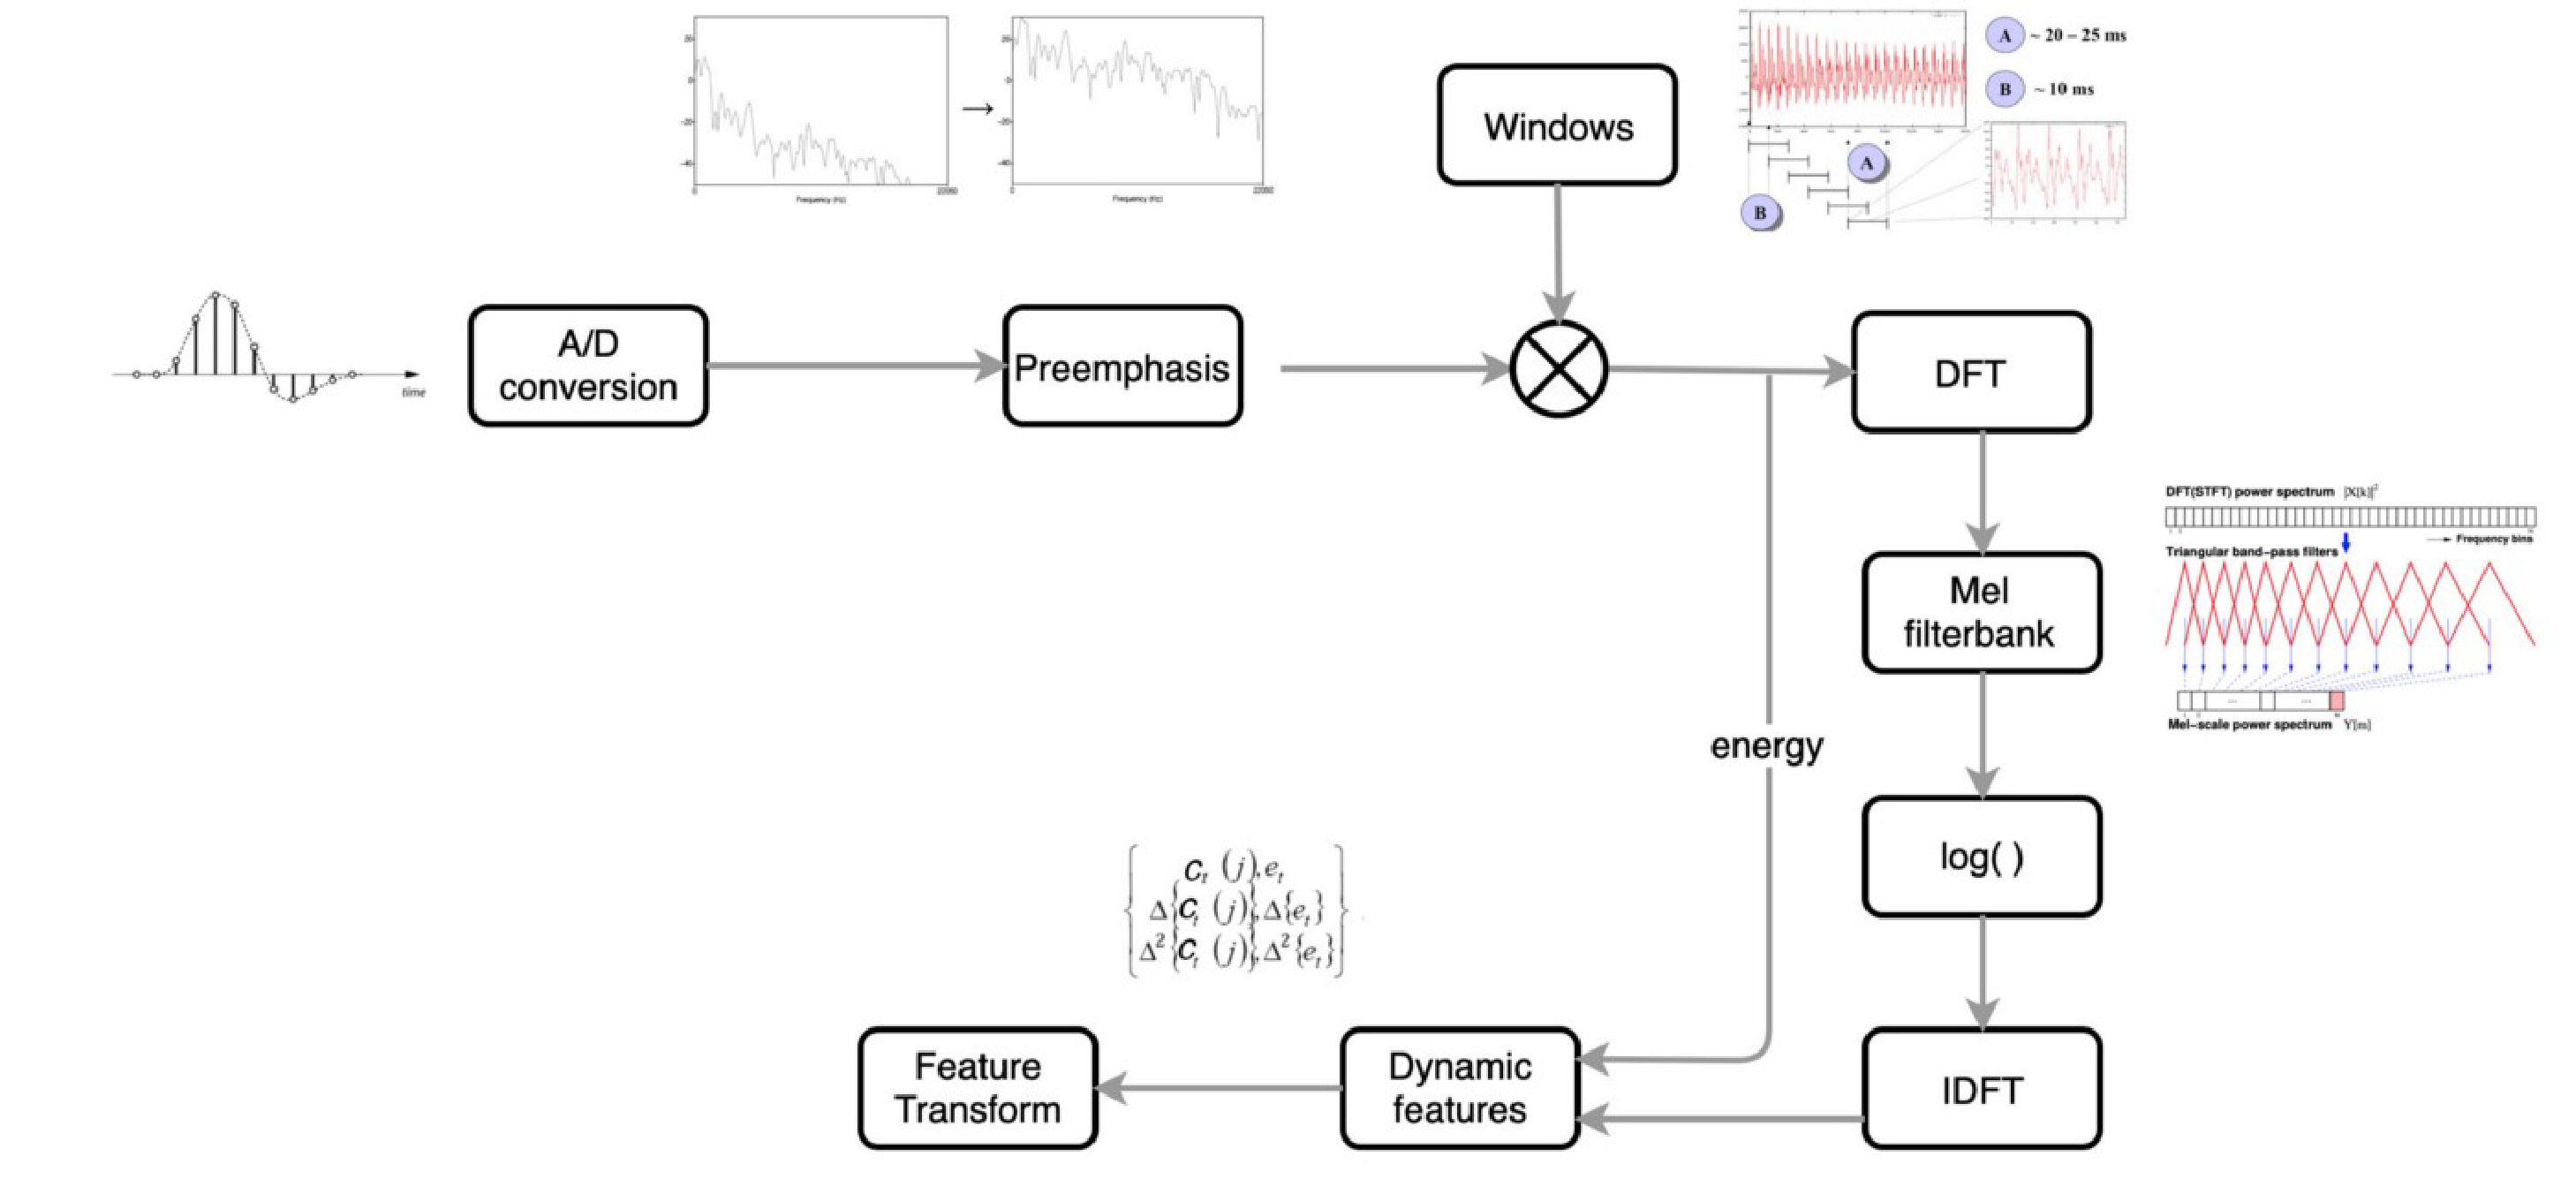
\includegraphics[width=1\textwidth]{resource/img/mfcc_flow.pdf}
        \caption{Tranform signal to MFCCs}
        \label{fig:LSTM}
    \end{minipage}
\end{figure}


\bibliographystyle{IEEEtran}
\bibliography{resource/references}
\end{document}
